\documentclass{article}

\usepackage{xspace}
\usepackage{amsmath}
\usepackage{afterpage}
\usepackage{stmaryrd}
\usepackage{graphicx,lipsum}
\usepackage{algorithm,algpseudocode}    
\usepackage{figlatex,wrapfig}
\usepackage[dvipsnames]{xcolor}
\usepackage{listings,amssymb,mathtools}
\usepackage{stmaryrd}
\usepackage{mathrsfs}
\usepackage{array,multirow}
\usepackage{pifont}
\usepackage{caption}
\usepackage{geometry}
\usepackage{textcomp}
\usepackage{tikz}
\usepackage{galois}

\usepackage{xspace}
\usepackage[colorlinks]{hyperref}
\hypersetup{
	colorlinks = true,
	citecolor = {violet},
	linkcolor = {MidnightBlue},
	urlcolor  = {MidnightBlue}
}


\newcommand{\mosc}{\texttt{memory\_order\_seq\_cst}\xspace}
\newcommand{\moacqrel}{\texttt{memory\_order\_acq\_rel}\xspace}
\newcommand{\morel}{\texttt{memory\_order\_release}\xspace}
\newcommand{\moacq}{\texttt{memory\_order\_acquire}\xspace}
\newcommand{\mocon}{\texttt{memory\_order\_consume}\xspace}
\newcommand{\morlx}{\texttt{memory\_order\_relaxed}\xspace}

\newcommand{\rf}[2]{{#1} {\color{Blue}\rightarrow^{rf}} {#2} }
\newcommand{\too}[2]{{#1} {\color{Blue}\rightarrow^{to}} {#2} }
\newcommand{\mo}[2]{{#1} {\color{Blue}\rightarrow^{mo}} {#2} }

\newcommand{\var}[1]{\color{OliveGreen}\texttt{#1}\color{black}}
\newcommand{\fun}[2]{\color{Sepia}\texttt{#1(\color{Gray}\textit{#2}\color{Sepia})}\color{black}}
\newcommand{\class}[1]{\color{DarkOrchid}\texttt{#1}\color{black}}

\date{}
\begin{document}
\title{Fence synthesis in C/C++11 programs}
\maketitle 

\section{Introduction} \label{sec:intro}
% ------------ INTRO PARAS ------------------
\par
A programmer working with relaxed memory constraints would want all the advantages of the relaxed model - such as speed and concurrency. However, using relaxed memory constraints comes with its own issues. In relaxed memory models, memory operations such as \textit{reads} and \textit{writes} can be reordered in order to achieve these properties. These instruction reorderings can cause certain variables to have different values in different execution runs of the same program, hence resulting in behaviour which is unexpected or surprising. These include not behaving according to sequentially consistent standards, or outputting unexpected values of variables.

\par
In this project, we suggest an approach to prevent certain unexpected behaviour, such as unexpected outputs due to concurrent instruction re-orderings in the C11 relaxed model.

\par
To tackle this, the programmer may add \textit{"assert"} statements in the source code, which will check that certain properties remain unchanged in each run of the program, such as the value of a variable in a certain thread. Each program will have several possibilities of runs where instructions will be executed in different orders. In some of these runs, there might be cases where the assertion does not hold and it gets violated. In the case that the \textit{assert} statement gets violated, the program execution will stop. The object of this project is to insert a minimum number of \textbf{C11 fences} in the source code of the program at the right places so that these assertions are satisfied and do not get violated.

% -------------------- MOTIVATION E.G. ------------------------
\subsection{Motivation Example}

% -------------------- FIG 1: BASIC ------------------------
\begin{figure}[!htb]
\begin{center}
\texttt{
init y := 0, x := 0;\\
	\begin{tabular}{c l || c l}
		(1) & y := 1 & (5) & x := 1\\
		(2) & if x == 0 & (6) & if y == 0\\
		(3) & \qquad c := 1 & (7) & \qquad c := 0\\
		(4) & \qquad t = c \color{olive}//1 & (8) & \qquad t = c \color{olive}//0
	\end{tabular}
}
	\caption{Simple two-thread dekker program}\label{fig:dekker1}
\end{center}
\end{figure}
\ishComment{to use R, W here as well? to show atomic operations? to use brackets for if?}

\par
In a sequentially consistent model, the multi-threaded program in Fig \ref{fig:dekker1} would execute the instructions in a sequentially consistent order. The final values read by variable \textit{t} would be 1 and 0 for each thread respectively. Therefore it can be said that the ``output'' would always be ``10''. However, in the case of a relaxed model, such as in a C11/C++11 program when all the instructions are relaxed, reading outputs of ``00'', ``01'', ``11'' may even be possible, thereby violating the rules of sequential consistency. Such an output may or may not be unexpected for the programmer, depending upon their requirements.

\par
For this reason, the programmer needs to provide their requirements about what values are expected at which locations by specifying a local safety property.

% --------------- FIG 2.2 basic + assert -------------
\begin{figure}[!htb]
\begin{center}
\texttt{
init y := 0, x := 0;\\
	\begin{tabular}{c l || c l}
		(1) & W$\mathtt{_{rel}}$y(1) & (5) & W$\mathtt{_{rel}}$x(1)\\
		(2) & if R$\mathtt{_{rel}x}$ == 0 & (6) & if R$\mathtt{_{rel}y}$ == 0\\
		(3) & \qquad W$\mathtt{_{rel}}$c(1) & (7) & \qquad W$\mathtt{_{rel}}$c(0)\\
		(4) & \qquad assert($\mathtt{R_{rel}c}$ == 1) & (8) & \qquad assert($\mathtt{R_{rel}c}$ == 0)
	\end{tabular}
}
	\caption{Simple two-thread dekker program in C11 syntax with assertions}\label{fig:dekker2}
\end{center}
\end{figure}

\par
Such a specification may be made in the form of assertions such as those described in Fig \ref{fig:dekker2} This ``assert'' statement checks that the expression provided to it holds at that point in the program. At the end of the threads, this safety property might not be satisfied. In this case, the program stops or exits, giving an error output. The objective of the tool to be created is to prevent the program from exhibiting behaviour which is unexpected for the programmer, hence preventing the error output as well as ensuring the provided specifications. For the purposes of this paper, we require the safety property to be specified as assertions in the program.

\section{An example}
\par
new

\section{The program}
\par
Order of events are as follows:
\begin{enumerate}
    \item The program has a main file which runs the tool in order, called \href{mainpy.tex}{\textit{main.py}} which take the input file from the user in the format \begin{center} \texttt{python main.py -f [filename].cc} \end{center} 
    
    \item This first takes the output from the model checking tool and translates the output into a list of all execution traces from the \href{translator.tex}{\textit{translator}} folder.
    
    \item This output is sent to \href{processing.tex}{\textit{processing.py}} where the data is processed and the required result is given. This result is in the form of list of possible locations where the fences can be inserted.
    
    \item The received output from \textit{processing.py} is sent to \textit{Z3} SAT/SMT Solver in order to obtain the optimal minimized number of fences. The output from this tool provides the exact fences and their locations to be inserted into the source program.
    
    \item The required locations obtained are then sent to \href{insert.tex}{\textit{insert.py}} where the fences are placed in the source program.
    
\end{enumerate}
\begin{figure}
    \centering
    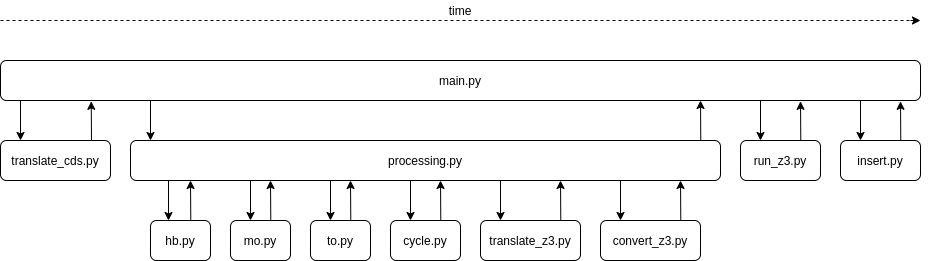
\includegraphics[width=0.9\textwidth]{img/time-flow.png}
    \caption{Order of operations in the tool}
\end{figure}
% TODO: create diagram depicting order of files IN LATEX
\section{Key}
\begin{itemize}
    \item \href{#4}{\textit{link}} denotes links to documents.
    \item \fun{function}{params} denotes functions.
    \item \var{variable } denotes variables.
    \item \class{class }denotes class names.
    \item The original program in which fences are to be inserted will be called "source program" and the tool made for this project will be referred to as "program" or "tool".
    \item A buggy execution trace as described by the model checker will be called "trace".
\end{itemize}

\end{document}